%%%%%%%%%%%%%%%%%%%%%%%%%%%%%%%%%%%%%%%%
%% HiMCM/MidMCM LaTeX Template -- 2026 %%
%% Problem B: Requirements 1 and 2 working draft
%% Revised after reviewing user-supplied 2025 B papers, November 7, 2026.
%%%%%%%%%%%%%%%%%%%%%%%%%%%%%%%%%%%%%%%%
\documentclass[12pt]{article}
\usepackage{geometry}
\geometry{left=1in,right=0.75in,top=1in,bottom=1in}
\newcommand{\Problem}{B}
\newcommand{\Team}{1111111} % Replace with the actual Team Control Number.
\usepackage{newtxtext}
\usepackage{amsmath,amssymb,amsthm}
\usepackage{newtxmath}
\usepackage[pdftex]{graphicx}
\usepackage{xcolor}
\usepackage{fancyhdr}
\usepackage{microtype}
\usepackage{xurl}
\usepackage{needspace}
\usepackage{booktabs,tabularx,array}
\usepackage[hidelinks]{hyperref}
\setlength{\headheight}{15pt}
\setlength{\parskip}{3pt}
\setlength{\parindent}{1.2em}
\lhead{Team \Team}
\rhead{}
\cfoot{}
\newtheorem{theorem}{Theorem}
\newtheorem{corollary}[theorem]{Corollary}
\newtheorem{lemma}[theorem]{Lemma}
\newtheorem{definition}{Definition}

\begin{document}
\graphicspath{{.}}
\DeclareGraphicsExtensions{.pdf,.jpg,.png}
\thispagestyle{empty}
\vspace*{-16ex}
\centerline{\begin{tabular}{*3{c}}
\parbox[t]{0.3\linewidth}{\begin{center}\textbf{Problem Chosen}\\ \Large \Problem\end{center}}&
\parbox[t]{0.3\linewidth}{\begin{center}\textbf{2026\\ HiMCM/MidMCM\\ Summary Sheet}\end{center}}&
\parbox[t]{0.3\linewidth}{\begin{center}\textbf{Team Control Number}\\ \Large \textcolor{red}{\Team}\end{center}}\\
\hline
\end{tabular}}

\begin{center}
\vspace{1.5em}
{\Large\bfseries Measuring Useful Cooling in Open Systems}\\[0.8em]
{\bfseries Working summary: Requirements 1 and 2}
\end{center}
An open freezer case must maintain appropriate product temperatures despite heat exchange with its surroundings. Electricity use alone does not show how well it performs this task.

We distinguish thermal demand, electrical input, and delivered storage service. Infiltration, cabinet heat transfer, internal equipment, restocking, and defrost contribute to demand. Equipment condition modifies performance, while temperature differences across product locations determine whether the intended service is delivered.

We identify four quantities that define cooling service efficiency: energy input, service quantity, local service quality, and service duration. Compliant product mass-hours per kilowatt-hour provide one possible freezer measure. Product-specific temperature requirements remain a separate adequacy check. Comparisons require prescribed loading, matched ambient conditions, and complete operating cycles.

We extend this principle to a regular-size New York City bus shelter, using documented dimensions and a three-zone model. Fan-driven air movement and evaporative temperature/humidity changes feed into a common SET-based hot-discomfort proxy. Signed relief accumulated over passenger-hours is divided by electrical energy, with remaining discomfort reported separately.

Six figures compare local conditions, electricity-normalized relief, humidity, passenger positions, delivery losses, and sensitivity. In the stated illustrative cases, the fan has the highest service efficiency, while the large evaporative cooler leaves the least residual discomfort. A delivery-loss stress test identifies conditions where the smaller evaporative cooler becomes more efficient. These are conditional scenario results, not measured device rankings. The power ratios give transparent break-even requirements: B and C must deliver respectively 4.8 and 10 times A's accumulated relief to exceed its service efficiency.

For Canberra MRT station, a three-zone dynamic model adds heat storage, moisture accumulation and time-dependent passenger loads. Device counts and allocation are evaluated against passenger demand through explicit service footprints. Matched simulations compare electricity, remaining discomfort and coverage to identify suitable equipment configurations. Documented architectural features are separated from assumed occupied area and operating parameters.

\medskip
\noindent\textit{Draft status.} Requirements 1 and 2 are developed here. Requirements 3--5 and the final whole-paper summary remain to be completed. Numerical results are simulations under explicit assumptions; no field performance measurements are claimed.

\clearpage
\pagestyle{fancy}
\rhead{Page \thepage}
\tableofcontents
\clearpage

\section{Understanding Cooling Efficiency}
\label{sec:understand}

An open freezer case succeeds by preserving its products. Low electricity use may reflect a smaller workload, shorter operation, or inadequate temperatures; high heat removal may reflect unwanted environmental heat gains. Cooling efficiency must therefore relate energy input to the storage service actually delivered.


Figure~\ref{fig:open-case} makes the open-front geometry concrete: the front opening permits air exchange, the cabinet surfaces transmit heat, and the shelves separate product locations whose temperatures should be checked. The pictured model is a medium-temperature refrigerated display case \cite{hillphoenix}; its geometry illustrates these mechanisms, while freezer operating temperatures and product requirements must be specified separately.

\begin{figure}[!ht]
\centering
\includegraphics[width=0.96\linewidth]{figures/09_open_display_case.pdf}
\caption{Open-front refrigerated display case: user-supplied schematic with external dimensions matching the Hillphoenix CF-R 4-ft configuration \cite{hillphoenix}. Millimetre labels are rounded; the internal shelf arrangement is schematic.}
\label{fig:open-case}
\end{figure}

\clearpage
\subsection{Selecting the quantities to evaluate}

Table~\ref{tab:service} identifies four quantities that enter the useful-service numerator or energy denominator in both settings.

\begin{table}[!ht]
\centering
\caption{Evaluation quantities and their transfer to a bus stop.}
\label{tab:service}
\small
\renewcommand{\arraystretch}{1.18}
\begin{tabularx}{\linewidth}{@{}>{\raggedright\arraybackslash}p{0.19\linewidth}
>{\raggedright\arraybackslash}X >{\raggedright\arraybackslash}X@{}}
\toprule
Quantity & Open freezer case & Bus-stop shelter\\
\midrule
Energy input & Electricity used by the case and its attributable refrigeration plant (kWh). & Electricity used by fans, pumps, and other cooling equipment (kWh).\\
Service quantity & Actual mass of products stored under a specified loading protocol (kg). & Number of people present in each occupied zone.\\
Local service quality & Product temperatures relative to product-specific storage requirements. & Thermal discomfort relative to the same setting without active cooling.\\
Service duration & Duration of product storage during the evaluation period (h). & Duration of passenger exposure while waiting (h).\\
\bottomrule
\end{tabularx}
\end{table}

\noindent\textbf{Energy input} includes auxiliaries and attributable plant electricity without overlapping meter readings. \textbf{Service quantity} accounts for workload, subject to prescribed loading limits.

\textbf{Local service quality} requires product temperatures at representative locations, rather than discharge-air temperature alone \cite{ashrae}. Averages can hide a warm shelf, and uniformity does not guarantee acceptable storage; product-temperature requirements remain essential \cite{etl}.

\textbf{Service duration} distinguishes sustained performance from a favorable snapshot. Include restocking, compressor cycling, and defrost recovery, with comparable initial and final thermal states so that stored cold cannot inflate the result.


\begin{figure}[!ht]
\centering
\includegraphics[width=\linewidth]{figures/00_cooling_service_process.pdf}
\caption{Process linking conditions to service and electricity over the same period ($E>0$).}
\label{fig:process}
\end{figure}

\clearpage
\subsection{Factors that explain performance}

Figure~\ref{fig:process} traces how operating conditions become delivered service. The arrows represent physical dependencies and service accounting; feedback and transient responses are handled within the later models. This process-oriented exposition draws on a supplied AI analysis, with the dependencies revised here \cite{gemini}.

\noindent\textbf{From surroundings to local conditions.} Infiltration carries sensible heat and moisture through the opening; walls transmit heat, and exposed surfaces exchange radiation. Geometry, insulation, ambient temperature, humidity, and airflow therefore alter the conditions around the products and the refrigeration demand \cite{ashrae}.

\noindent\textbf{From operation to local conditions.} Lights and fans release heat, warmer incoming stock adds a temporary load, and defrost interrupts normal cooling \cite{ashrae}. Equipment condition changes insulation, airflow, and power demand. These mechanisms affect both local conditions and measured electricity; age itself is not an additional score.

\noindent\textbf{From local conditions to service.} Product placement and thermal response determine whether the food remains within its required range. Accumulating compliant product mass over time gives useful storage service. The same sequence applies to passengers, but their response depends on the thermal environment and their exposure, rather than food-temperature limits.

\subsection{Implications for the bus-stop model}

The preceding analysis motivates a common evaluation principle:
\begin{equation}
\boxed{\text{Cooling efficiency}
=\frac{\text{useful service accumulated over objects and time}}
{\text{energy input over the same period}}.}
\label{eq:principle}
\end{equation}

The freezer measure can be expressed in compliant kg\,h per kWh. At a bus stop, useful service accumulates thermal-discomfort reduction over people and waiting time. The next model specifies this response and spatial calculation; the two settings do not have numerically comparable units.

First, \textbf{evaluate people directly}. A fan changes local air movement and can improve thermal sensation without lowering air temperature \cite{energystar}. A direct evaporative cooler changes temperature and humidity \cite{evap}. Device-specific mechanisms therefore feed into a common assessment of passenger response.

Second, \textbf{weight effects by occupancy}. Geometry and airflow determine which occupied zones benefit; cooling empty space receives no passenger-service credit. Area is not multiplied by total headcount again. Outdoor air exchange may disperse cooled air while changing local air movement, so its effect is assessed through passenger response.

Third, \textbf{retain a minimum-service check}. Check individual product-temperature excursions and remaining unacceptable passenger exposure even when aggregate service is high. Partial relief can count as a benefit without establishing adequacy; minimum requirements remain separate from the efficiency score.

Within a venue, compare strategies under matched weather, occupancy, geometry, and evaluation periods. Water use, operating cost, and broader visitor experience enter the later effectiveness model. AI-assisted analysis and drafting are recorded in the appended report \cite{codex}.

\clearpage
\section{Cooling a Bus Stop: From Local Conditions to Passenger Service}
\label{sec:bus}

We apply the service principle in Section~\ref{sec:understand} to Requirement 2(a). A device first changes the environment at each passenger's position; those changes alter thermal discomfort; the resulting relief is accumulated over people and time. This separates three questions: how much relief is delivered, where it is delivered, and how much electricity it requires.


We adopt the regular-size New York City shelter in Figure~\ref{fig:shelter-geometry} as the common geometry for all three devices. Its documented dimensions provide a reproducible physical scale for the occupied zones.

\begin{figure}[!ht]
\centering
\includegraphics[width=\linewidth]{figures/07_bus_shelter_geometry.pdf}
\caption{Adopted baseline geometry: regular-size New York City bus shelter. User-supplied schematic; dimensions verified against NYC DOT's \emph{Street Design Manual} \cite{nycshelter}. Millimetre labels are rounded.}
\label{fig:shelter-geometry}
\end{figure}

The official dimensions are $14$ ft by $5$ ft by $8$ ft $11$ in \cite{nycshelter}. Converting the imperial values before rounding gives $L=4.2672$, $W=1.5240$, and $H=2.7178$ m. We use the gross plan area $A=LW=6.5032\,\mathrm{m^2}$ and divide the length into three equal strips, each with $A_z=A/3=2.1677\,\mathrm{m^2}$. The bench and structure occupy part of this footprint; $A$ is a geometric reference, not a net standing area or a capacity estimate.

\begin{figure}[!ht]
\centering
\includegraphics[width=\linewidth]{figures/08_shelter_zoning.pdf}
\caption{Calculation zones derived from the adopted dimensions. Equal strips and the delivery reference at $x=0$ are modeling choices; dots mark representative zone coordinates, not passenger locations. No bench or obstruction dimensions are inferred.}
\label{fig:shelter-zones}
\end{figure}

Figure~\ref{fig:shelter-zones} fixes the spatial interpretation of near, middle, and edge. Their representative coordinates are $(x_z,W/2)$, with $x_z=(z-\tfrac12)L/3$ for $z=1,2,3$. We assume delivery originates at the $x=0$ end and use the zone-average fields in Table~\ref{tab:bus-fields}. This is a defined layout for comparison; the dimensions alone do not determine air speed or cooling reach.

\subsection{Data, interpretation, and a reproducible scenario}

The problem describes A as a fan with an apparent cooling effect of up to $3\,^{\circ}\mathrm C$, and B and C as evaporative coolers with air-temperature reductions of up to $5$ and $8\,^{\circ}\mathrm C$ \cite{problem}. These effects use different temperature concepts. We do not subtract $3\,^{\circ}\mathrm C$ from the air temperature for A or treat its unspecified ``feels like'' index as measured SET.

The table labels energy use in kW/hr. To obtain a dimensionally consistent comparison, \textbf{we interpret its numerical entries as mean operating powers} $P_A=0.25$, $P_B=1.2$, and $P_C=2.5$ kW. Thus a one-hour comparison uses $0.25$, $1.2$, and $2.5$ kWh. This is a stated interpretation, not a verified correction to equipment specifications.

The problem supplies no airflow, coverage map, rating weather, or evaporative effectiveness. Therefore, the numerical analysis below is an \textbf{illustrative scenario analysis, not an identification of actual device performance}. Table~\ref{tab:bus-assumptions} specifies the common environment; Table~\ref{tab:bus-fields} specifies the uncertain delivered fields before comparing outcomes.

\begin{table}[!ht]
\centering\small
\caption{Common inputs: documented geometry and explicit scenario assumptions.}
\label{tab:bus-assumptions}
\renewcommand{\arraystretch}{1.12}
\begin{tabularx}{\linewidth}{@{}p{0.31\linewidth}X@{}}
\toprule
Quantity & Value, basis, and interpretation\\
\midrule
Shelter & NYC regular-size geometry: $4.2672\times1.5240\times2.7178$ m \cite{nycshelter}; three equal $2.1677\,\mathrm{m^2}$ gross zones. Full shade is assumed.\\
Weather & $T_a=34\,^{\circ}\mathrm C$; dry/humid cases RH $=30/70\%$; sweep $20$--$80\%$.\\
Radiation and background air & Mean radiant temperature $T_r=36\,^{\circ}\mathrm C$; baseline local speed $v_0=0.20$ m/s; pressure $101325$ Pa.\\
Reference passenger & Standing, $1.2$ met, $0.5$ clo; default body area $1.8258\,\mathrm{m^2}$ and zero external work in the SET implementation.\\
Occupancy and period & Assumed mean simultaneous occupancy $(4,4,4)$ over one hour: $12$ person-hours; an illustrative load, not a measured count or rated capacity.\\
Alternative distributions & Concentration stress cases $(8,3,1)$ and $(1,3,8)$; both retain the same total of 12 people.\\
Decision threshold & SET threshold $\Theta_c=26\,^{\circ}\mathrm C$, an assumed hot-discomfort reference; tested at $24$ and $28\,^{\circ}\mathrm C$.\\
\bottomrule
\end{tabularx}
\end{table}

\begin{table}[!ht]
\centering\small
\caption{Assumed local delivery profiles. Entries follow near/middle/edge order.}
\label{tab:bus-fields}
\begin{tabularx}{\linewidth}{@{}lXXc@{}}
\toprule
Device & Local air speed (m/s) & Cooled-air mass fraction $f_{s,z}$ & $\varepsilon_s$\\
\midrule
A & $1.00 / 0.55 / 0.25$ & $0 / 0 / 0$ & ---\\
B & $0.80 / 0.50 / 0.30$ & $0.80 / 0.45 / 0.10$ & $0.70$\\
C & $1.00 / 0.80 / 0.50$ & $0.90 / 0.70 / 0.40$ & $0.70$\\
\bottomrule
\end{tabularx}
\end{table}

The entries represent zone averages over the strips in Figure~\ref{fig:shelter-zones}; they are not measured NYC delivery data. Here $f_{s,z}$ is the local dry-air mass mixing fraction of treated air, not a division of the device's total flow among zones; its three entries need not sum to one. The larger coverage assumed for C is tested, not presented as a fact supplied by the problem.

\subsection{Predicting the local environment}

\noindent\textbf{Fan A: air movement.} We set $T_{A,z}=T_a$ and retain ambient moisture, while prescribing local speeds from Table~\ref{tab:bus-fields}. The resulting convection and evaporation enter the passenger-response model. This follows the physical distinction between moving air and lowering dry-bulb temperature \cite{fanguide}. We neglect the fan motor's small local heat plume in this open, mixed-air approximation.

\noindent\textbf{B and C: evaporation followed by dilution.} Direct evaporation reduces dry-bulb temperature while increasing moisture; the entering wet-bulb temperature $T_{wb}$ limits the achievable depression \cite{evapequip}. We adopt
\begin{equation}
 T_{o,s}=T_a-\min\{\Delta T_s^{\max},\;\varepsilon_s(T_a-T_{wb})\},
 \qquad s\in\{B,C\},
\label{eq:outlet}
\end{equation}
where $\Delta T_B^{\max}=5$ and $\Delta T_C^{\max}=8\,^{\circ}\mathrm C$. Applying these advertised shelter-temperature reductions as outlet caps is an explicit modeling convention; the problem does not specify their measurement location. The caps do not imply that either device achieves them under every climate.

Let $w$ denote kg of water vapor per kg of dry air and $h$ the moist-air enthalpy in kJ/kg of dry air. Using standard SI psychrometric relations \cite{psychrolib},
\begin{align}
 w&=0.621945\frac{p_v}{p-p_v},\qquad p_v=\phi p_{sat}(T),\\
 h(T,w)&=1.006T+w(2501+1.86T),
\label{eq:enthalpy}
\end{align}
where $\phi$ is RH as a fraction. Approximating evaporation as isenthalpic, $h_{o,s}\simeq h_a$, gives
\begin{equation}
 w_{o,s}=\frac{h_a-1.006T_{o,s}}{2501+1.86T_{o,s}}.
\end{equation}
This neglects fan heat and make-up-water enthalpy; near-constant enthalpy is not an assertion of exact constant wet-bulb temperature \cite{evap}.

Outdoor dilution is represented by a two-stream balance on dry-air mass:
\begin{align}
 w_{s,z}&=(1-f_{s,z})w_a+f_{s,z}w_{o,s},\\
 h_{s,z}&=(1-f_{s,z})h_a+f_{s,z}h_{o,s},\\
 T_{s,z}&=\frac{h_{s,z}-2501w_{s,z}}{1.006+1.86w_{s,z}}.
\label{eq:mixing}
\end{align}
We recover RH from $T_{s,z}$ and $w_{s,z}$, rather than averaging RH directly. Every calculated state is checked against saturation. This reduced model needs measured local delivery profiles for site-specific predictions; it is not a CFD calculation.

\subsection{Converting local conditions to a common human response}

We compute standard effective temperature (SET), denoted $\Theta$, from
\begin{equation}
 \Theta_{s,z}=F_{\mathrm{SET}}(T_{s,z},T_{r,z},v_{s,z},\phi_{s,z};\mathrm{met},\mathrm{clo}).
\label{eq:set}
\end{equation}
SET compares physiological heat exchange with that in a reference environment, making it more suitable here than air-temperature drop alone \cite{thermalcomfort,fanguide}. We use the published \texttt{pythermalcomfort} implementation with input-domain checks enabled \cite{pythermal}. All scenario inputs remain inside its documented temperature, air-speed, clothing, and activity limits. SET is used as a quasi-steady engineering comparison: its reference conditions originate in typical indoor applications, and it does not model a passenger's prior walking or individual transient response \cite{thermalcomfort}.

\subsection{Measuring service and retaining a quality check}

For the warm-weather scenarios, define the hot-discomfort proxy
\begin{equation}
 D(\Theta)=[\Theta-\Theta_c]_+,\qquad [x]_+=\max(x,0).
\end{equation}
The threshold is a decision assumption, not an ASHRAE safety limit. Let $0$ denote the same shelter without active cooling, retaining the same shade, weather, radiation, and background air movement. The signed local improvement is
\begin{equation}
 b_{s,z,k}=D(\Theta_{0,z,k})-D(\Theta_{s,z,k}).
\end{equation}
Negative values are retained: an adverse condition must reduce useful service. Over time steps of $\Delta t_k$ hours,
\begin{align}
 U_s&=\sum_k\sum_z n_{z,k}b_{s,z,k}\Delta t_k, &
 E_s&=\sum_k P_{s,k}\Delta t_k,\\
 \eta_s&=U_s/E_s,\qquad E_s>0.
\label{eq:bus-efficiency}
\end{align}
The unit of $\eta$ is person$\cdot{}^{\circ}\mathrm C\cdot$h/kWh, with temperature measured on the SET scale. This is a service-efficiency index, not a thermodynamic percentage or COP. Empty zones earn no credit, although operating electricity is still counted. The zero-energy baseline has no efficiency ratio.

We also report remaining discomfort,
\begin{equation}
 R_s=\sum_k\sum_z n_{z,k}D(\Theta_{s,z,k})\Delta t_k,
 \qquad \overline D_s=\frac{R_s}{\sum_k\sum_z n_{z,k}\Delta t_k}.
\label{eq:remaining}
\end{equation}
A high $\eta_s$ alone does not establish adequate relief. If a decision-maker specifies an acceptable residual or an individual exposure requirement, it should be imposed separately; no universal heat-health threshold is inferred from our SET proxy. When the baseline already meets the chosen hot-discomfort criterion, further cooling earns no benefit, and switching off can be appropriate.

\noindent\textbf{How geometry enters service accounting.} The code derives each $A_z$ and its coordinates from $L$ and $W$. Occupancy may be supplied directly as $n_z$, as in our comparison, or through a gross-area reference density $\rho_z$, giving $n_z=\rho_zA_z$. The uniform case corresponds to $12/A=1.8452$ persons per gross square metre. Concentrating eight people in one strip gives $8/A_z=3.6905$; this is an abstract crowd-concentration stress case, not a demonstrated feasible standing layout. A deployable layout requires bench and circulation dimensions and revised occupancies.

Area is therefore counted once through population when density is the input. Multiplying $U_s$ by area or total headcount again would double-count service. With headcounts and local fields held fixed, changing geometric dimensions alone leaves $U_s$ unchanged; with gross-area densities and local fields fixed, service scales with area. Both statements are accounting properties, not predictions that airflow is unaffected by shelter size. Increasing every $n_z$ by a common factor cannot change ranking under fixed local conditions.

\noindent\textbf{A ranking result independent of the assumed delivery maps.} Under the interpreted constant powers and a common operating period,
\begin{equation}
\begin{aligned}
 \eta_B>\eta_A&\iff U_B>4.8U_A,\\
 \eta_C>\eta_A&\iff U_C>10U_A,\\
 \eta_C>\eta_B&\iff U_C>\frac{25}{12}U_B.
\end{aligned}
\label{eq:break-even}
\end{equation}
Thus nominal temperature reduction alone cannot justify a larger device. Its accumulated passenger relief must compensate for its larger electricity input. These inequalities follow from the given power ratios; their validity does not depend on the assumed zone profiles.

\subsection{Numerical results: local mechanisms and the efficiency tradeoff}

\begin{figure}[!ht]
\centering
\includegraphics[width=\linewidth]{figures/01_local_conditions.pdf}
\caption{Simulated local air temperature, RH, and SET under the stated assumptions. Fan A leaves air temperature unchanged while changing SET. B and C lower air temperature and increase RH. These are scenario outputs, not field measurements.}
\label{fig:bus-local}
\end{figure}

Spatial delivery matters even within one small shelter. In the dry case, C gives SET $26.3\,^{\circ}\mathrm C$ near the outlet but $29.4\,^{\circ}\mathrm C$ at the edge. At RH $70\%$, these become $33.1$ and $35.2\,^{\circ}\mathrm C$. A single mean air-temperature reduction would conceal these differences. A, meanwhile, improves SET without changing the $34\,^{\circ}\mathrm C$ dry-bulb temperature.

\begin{figure}[!ht]
\centering
\includegraphics[width=\linewidth]{figures/02_efficiency_and_quality.pdf}
\caption{Uniform occupancy: electricity-normalized relief and remaining hot-discomfort proxy. Lower residual is better, whereas higher service efficiency is better. The $26\,^{\circ}\mathrm C$ SET reference is assumed.}
\label{fig:bus-quality}
\end{figure}

For uniform occupancy, dry-case efficiencies are $84.6$, $24.5$, and $21.1$ for A, B, and C, respectively. Yet their mean remaining SET excesses are $4.40$, $3.72$, and $1.76\,^{\circ}\mathrm C$: C delivers more total relief while A delivers more per kWh. At RH $70\%$, efficiencies are $90.6$, $21.1$, and $15.2$; even C retains a mean excess of $8.05\,^{\circ}\mathrm C$. The efficiency winner therefore does not establish that the shelter meets a comfort or safety requirement.

\subsection{Climate and passenger distribution}

\begin{figure}[!ht]
\centering
\includegraphics[width=\linewidth]{figures/03_humidity_sweep.pdf}
\caption{RH sweep with temperature, radiation, occupancy, and delivery profiles fixed. Outlet cooling is bounded by both the specified cap and the wet-bulb depression.}
\label{fig:bus-humidity}
\end{figure}

The assumed outlet drops change from $5/8\,^{\circ}\mathrm C$ for B/C in the dry case to approximately $3.4/3.4\,^{\circ}\mathrm C$ in the humid case. Their common high-humidity outlet temperature follows from the shared assumed $\varepsilon=0.7$ once neither cap is active; it is not a measured equality between the devices. Remaining performance differences then come from their delivery profiles. Service efficiency need not vary monotonically with RH because SET includes nonlinear human heat exchange and the baseline also changes. Air movement can still provide relief when evaporative temperature reduction weakens.

\begin{figure}[!ht]
\centering
\includegraphics[width=\linewidth]{figures/04_occupancy.pdf}
\caption{Moving the same 12 mean occupants between near, middle, and edge zones changes delivered service. Labels give the three zone occupancies.}
\label{fig:bus-occupancy}
\end{figure}

In dry conditions, A's efficiency falls from $118.3$ under near-heavy occupancy to $48.3$ under edge-heavy occupancy. More importantly, the B/C ordering reverses: under uniform occupancy B exceeds C ($24.5$ versus $21.1$), while at the edge-heavy stop C exceeds B ($16.6$ versus $15.5$). The same total population is being served; the change comes from where people stand relative to the assumed delivery fields. A remains the most energy-efficient option in all six nominal climate--occupancy cases.

\subsection{When the recommendation changes}

A poorly aimed or obstructed fan can consume electricity without delivering its nominal air movement to passengers. We test this specific failure mode using
\begin{equation}
 v_{A,z}(q)=v_0+q(v_{A,z}^{\mathrm{nom}}-v_0),\qquad 0\leq q\leq1,
\end{equation}
while holding $P_A=0.25$ kW. Here $q$ describes delivery loss at occupied positions, \emph{not} a fan-speed control setting; changing motor speed would require a different power model. The B/C profiles stay fixed in this particular stress test.

\begin{figure}[!ht]
\centering
\includegraphics[width=\linewidth]{figures/05_delivery_decision.pdf}
\caption{Conditional efficiency winner on the complete RH--fan-delivery grid: RH $20$--$80\%$ in one-percentage-point steps and $q=0$--$1$ in steps of $0.02$. The boundary is grid-resolved. This tests fan delivery loss; it is not a universal climate-selection map.}
\label{fig:bus-decision}
\end{figure}

The first sampled $q$ at which A wins is $0.18$ at RH $30\%$ and $0.16$ at RH $70\%$; the corresponding switch lies between that sample and the preceding $0.02$ grid step. At lower delivery, B wins. C has no winning cells in this particular grid, although it provides greater absolute relief in the nominal cases. Every humidity column has one contiguous A-winning interval. These boundaries depend on the prescribed B/C fields and are not real-world probabilities or universal fan-performance thresholds.

\noindent\textbf{Operational interpretation.} First preserve shade and place people within useful airflow. Compare the measured benefit of improving equipment placement with the benefit of adding cooling capacity. If a larger evaporative system serves substantially more occupied space, use Eq.~\eqref{eq:break-even} with its measured service to decide whether that expansion compensates for electricity use. In humid conditions, an assumed larger nominal temperature drop cannot override the wet-bulb constraint.

A field calibration would measure $(T,\mathrm{RH},v,T_r)$ at occupied positions within the documented strips, electricity over the same period, and occupancy by zone. Net usable area and actual device placement would also be recorded. Repeated matched weather and occupancy conditions would allow the assumed profiles in Table~\ref{tab:bus-fields} to be replaced and the ranking checked. The quoted $3/5/8\,^{\circ}\mathrm C$ effects alone cannot supply this calibration.

\subsection{Sensitivity, verification, and scope}

\begin{figure}[!ht]
\centering
\includegraphics[width=\linewidth]{figures/06_sensitivity.pdf}
\caption{One-factor-at-a-time sensitivity at the two endpoint settings listed on each row; dots mark nominal ratios. An interval above one would favor the evaporative device over A. These are assumed parameter ranges, not statistical confidence intervals. Joint uncertainty can produce changes beyond these endpoint tests.}
\label{fig:bus-sensitivity}
\end{figure}

Across the tested individual endpoint changes, the largest B/A and C/A efficiency ratios are $0.432$ and $0.372$; no endpoint reverses the nominal advantage of A. This does not prove robustness over every intermediate value or joint parameter combination. Added-speed factors scale $v-v_0$, and cooled-air fractions are capped at one. The rating-interpretation test removes the $5/8\,^{\circ}\mathrm C$ outlet caps while retaining the wet-bulb constraint; it addresses uncertainty in where the quoted temperature effects were measured. The delivery-loss test in Figure~\ref{fig:bus-decision} already demonstrates that stronger departures can change the winner.

\noindent\textbf{Verification.} The implementation checks psychrometric round trips, dry-air moisture/enthalpy mixing balances, wet-bulb bounds, and saturation. Service-accounting checks verify $U_s+R_s=R_0$, zero benefit at zero occupancy, zero benefit when all delivered effects vanish, and unchanged rankings when every zone's population doubles. A signed-adverse-effect check confirms that worsening discomfort is not clipped away. No credit is given for additional cooling of an already comfortable baseline. Geometry checks verify unit conversion and area conservation, equivalence of count and density inputs, fixed-count invariance, and fixed-density scaling under unchanged local fields.

\Needspace{4\baselineskip}
\noindent\textbf{Limitations and transfer.} Local profiles and representative passengers remain assumptions; the numerical ranking is conditional on them. Airflow and dilution are prescribed rather than solved from fan curves, mass flow, crosswind, and shelter geometry. Radiation is fixed for a shaded shelter, so direct sun and changing shadow patterns need additional modeling. Short waiting times and varied physiological histories are not resolved by quasi-steady SET. Without measured flow, water consumption cannot be calculated reliably from the moisture increase alone; water and operating cost belong in the later effectiveness analysis. Section~\ref{sec:rail} retains this service accounting and adds surface heat storage and dynamic air/moisture exchange for a semi-open station.

\noindent\textbf{Reproducibility.} Calculations use \texttt{pythermalcomfort} 4.8.1 and PsychroLib 2.5.0. The accompanying \texttt{model} folder contains the sourced geometry, scenario assumptions, psychrometric/SET backend, executable simulation, CSV outputs, and source audit. A geometry audit records zone coordinates, areas, and implied occupancies; six numerical figures and the zoning diagram have reproducible source code. Each figure is loaded from a separate PDF in the \texttt{figures} folder, allowing independent replacement. Software versions and checks are saved with the results. Simulations quantify the stated assumptions; they do not constitute experimental validation.

\clearpage
\section{Canberra MRT Station: A Semi-open Waiting-area Case}
\label{sec:rail}

\subsection{Site evidence and the modeled waiting area}

We select Canberra MRT station in Singapore for Requirement 2(b). RSP describes an elevated, two-storey station with a site area of $9,128\,\mathrm{m^2}$ \cite{canberra-rsp}. LTA identifies platform planting, daylight-admitting glazing and rain-protective louvers that allow natural ventilation \cite{canberra-lta}. The design question is which device types, quantities and locations can meet passenger cooling and coverage requirements with the least electricity. We evaluate candidate installations of A, B and C in this shaded, humid, semi-open setting; their deployment is hypothetical.

\begin{figure}[!ht]
\centering
\includegraphics[width=0.96\linewidth]{figures/13_canberra_station.pdf}
\caption{User-supplied Canberra station schematic, retained as a separate PDF. Approximate structural dimensions are contextual references; the drawing is not an as-built survey or a map of the calculation zones. Sources identified in the drawing are listed in \cite{canberra-dimensions,canberra-rsp}.}
\label{fig:canberra}
\end{figure}

\noindent\textbf{Geometry and scope.} Figure~\ref{fig:canberra} labels approximately 220 m station length, roof-truss span over 28 m, and roughly 17 m columns. The column height is not platform-to-roof clearance; the roof span includes non-waiting space. Neither their product nor the site area specifies the occupied air volume. We instead define an explicit station-scale planning scenario. Taking the approximately 220 m length as a reference, assume an aggregate waiting-strip width $b=6$ m and usable fraction $\alpha=0.8$, giving
\begin{equation}
 A_{\mathrm{occ}}=\alpha Lb=1056\,\mathrm{m^2}.
\label{eq:canberra-area}
\end{equation}
Neither $b$ nor $\alpha$ is measured: they represent waiting space after excluding tracks, access obstructions and non-waiting portions. Three equal aggregate zones of $352\,\mathrm{m^2}$ represent access-side, sheltered-core and exposed-edge conditions. Their assumed effective mixing height is 4 m, giving $1408\,\mathrm{m^3}$ per zone. These are functional control volumes, not surveyed platform compartments. This formulation uses the station's scale without treating column height or site area as occupied volume.

\subsection{What changes from the bus model, and why}

The service objective is unchanged. The station roof and partial enclosure motivate air and surface storage, while recirculation can accumulate moisture. Passenger arrivals and boarding alter both heat loads and demand over time. We replace prescribed temperature/humidity fields with coupled zone balances. The site's greenery is not assigned an unsupported numerical cooling credit; its effect would enter measured surface temperatures and envelope parameters.

\begin{table}[!ht]
\centering\small
\caption{Revisions to the bus model and their purpose.}
\label{tab:rail-changes}
\begin{tabularx}{\linewidth}{@{}>{\raggedright\arraybackslash}p{0.25\linewidth}>{\raggedright\arraybackslash}X>{\raggedright\arraybackslash}X@{}}
\toprule
Revision & Why it is needed & Added capability\\
\midrule
Air and surface storage & Partial enclosure allows thermal memory. & Predict warm-up, lag and residual heat.\\
Dynamic moisture and zone exchange & Recirculation changes inlet humidity; openings connect different regions. & Calculate evaporative feedback and dilution.\\
Time-dependent passengers & Arrivals and boarding change both loads and service demand. & Count time-resolved person-hours and crowd heat/moisture.\\
Device counts and service coverage & Cooling demand and passenger density vary across a large station. & Select quantities and locations using total power and passenger service.\\
\bottomrule
\end{tabularx}
\end{table}

\subsection{Coupled heat, moisture, and surface balances}

Following the control-volume structure of building heat and moisture balances \cite{epzone}, let each zone store moist-air enthalpy $h_z$ (J/kg dry air), humidity ratio $w_z$ (kg/kg dry air), and an effective roof/wall inner-surface temperature $T_{m,z}$. The air is well mixed within each zone. Its dry-air mass is approximated as constant, $M_z=\rho_{da,o}V_z$, with outdoor reference density. This is a reduced model, not an EnergyPlus or CFD simulation.

Define the exchange operator, for either $x=h$ or $w$, as
\begin{equation}
 \mathcal L_z(x)=\dot m_{0z}(x_o-x_z)+\sum_{j\ne z}\dot m_{zj}(x_j-x_z),
 \qquad \dot m_{0z}=M_z\lambda_z/3600.
\label{eq:rail-exchange}
\end{equation}
Here $\lambda_z$ is the assumed outdoor air-change rate in h$^{-1}$. Each exchange represents equal entering and leaving dry-air flow; adjacent-zone rates satisfy $\dot m_{zj}=\dot m_{jz}$. Wind, buoyancy and opening geometry can affect outdoor exchange \cite{ventilation}; a prescribed train-cycle pulse tests that uncertainty without claiming a station-specific piston-flow law.

With $x_{zk}$ devices of type $k$ in zone $z$, unit recirculation $\dot m_k$ (kg dry air/s), and time in seconds, our balances are
\begin{align}
 M_z\dot h_z={}&\mathcal L_z(h)+H_{ma,z}(T_{m,z}-T_z)
 +n_zq_c+n_zg h_v(T_z)+P_z
 +\sum_k x_{zk}\dot m_k(h_{e,zk}-h_z),\label{eq:rail-enthalpy}\\
 M_z\dot w_z={}&\mathcal L_z(w)+n_zg+
 \sum_k x_{zk}\dot m_k(w_{e,zk}-w_z),\label{eq:rail-moisture}\\
 C_{m,z}\dot T_{m,z}={}&H_{mo,z}(T_o-T_{m,z})+Q_{\mathrm{sol},z}
 +n_zq_r-H_{ma,z}(T_{m,z}-T_z).\label{eq:rail-surface}
\end{align}
The per-person inputs are convective heat $q_c$, radiative heat $q_r$, and water-vapor generation $g$. Vapor enters with $h_v(T)=2501000+1860T$ J/kg; no additional latent-heat term is added. Total device power $P_z=1000\sum_k x_{zk}p_k$ (W), with unit powers $p_k$ in kW, is assumed to dissipate locally as sensible heat. Pump power is already included in the device total. Conductances $H$ have units W/K, surface capacity $C_m$ has units J/K, and $Q_{\mathrm{sol}}$ is an effective absorbed envelope load. The opposite signs of the air--surface term conserve internal energy.

Air temperature is recovered from $T_z=(h_z-2501000w_z)/(1006+1860w_z)$. A shaded longwave approximation for the surface contribution to comfort \cite{thermalcomfort} gives
\begin{equation}
 T_{r,z}=\left[F_z(T_{m,z}+273.15)^4+(1-F_z)(T_{r,o}+273.15)^4\right]^{1/4}-273.15.
\label{eq:rail-mrt}
\end{equation}
$F_z$ is an assumed effective view fraction; the example sets external radiant temperature $T_{r,o}=T_o$, while keeping it a separate input. Direct sun on passengers and detailed radiative asymmetry are excluded.

\noindent\textbf{Device mechanisms.} A adds air movement and electrical heat, with $\dot m_A=0$. B/C recirculate local air: at every step Eq.~\eqref{eq:outlet} is evaluated using the \emph{current zone inlet}, rather than fixed outdoor conditions. Their approximate outlet enthalpy remains $h_{e,zk}=h_z$, while $w_{e,zk}>w_z$ when evaporation occurs. Thus evaporation can lower dry-bulb temperature without removing moist-air enthalpy. Rising local moisture reduces subsequent wet-bulb depression. The earlier fixed mixing fractions are replaced by these explicit flow balances. Local passenger air speeds remain stated assumptions, rather than solutions of a momentum model.

\subsection{Equipment selection, allocation, and coverage}

Let $x_{zk}\in\mathbb Z_{\ge0}$ be the number of devices of type $k\in\{A,B,C\}$ in zone $z$. A $3\times3$ count matrix specifies a candidate installation, allowing quantities and device types to vary by zone. Each candidate is evaluated through the resulting shared thermal environment: all operating units contribute heat and electricity, and evaporative units also contribute moisture.

We use assumed, non-overlapping service footprints $a_A=20$, $a_B=30$ and $a_C=40\,\mathrm{m^2}$ per unit. These are comparison inputs, not manufacturer coverage ratings. For uniform passenger density within a zone, define
\begin{equation}
 f_{zk}=\frac{x_{zk}a_k}{A_z},\qquad
 f_{z0}=1-\sum_k f_{zk}\ge0,\qquad \sum_kx_{zk}a_k\le A_z.
\label{eq:coverage}
\end{equation}
The uncovered fraction experiences local speed $v_0$; each covered subgroup experiences its device-specific speed $v_{zk}$. We average \emph{discomfort}, not velocities or device efficiencies:
\begin{equation}
 \overline D_{s,z}(t)=f_{z0}D[\Theta(T_z,T_{r,z},v_0,\phi_z)]
 +\sum_k f_{zk}D[\Theta(T_z,T_{r,z},v_{zk},\phi_z)].
\label{eq:mixed-discomfort}
\end{equation}
All subgroups share the zone's mixed temperature, humidity and radiant environment; an uncovered passenger can therefore still experience indirect cooling or humidification. The coverage fraction measures direct air-movement service, not a boundary of all thermal influence. The formulation represents distributed equipment with separate service footprints. Co-located jets, overlapping footprints and series arrangements require a resolved airflow model.

\subsection{Canberra scenario and comparable deployment tests}

We assume $33\,^{\circ}\mathrm C$ and $70\%$ outdoor RH for a hot, humid Canberra scenario. Singapore's weather service describes typical daytime maxima of $31$--$33\,^{\circ}\mathrm C$ and high humidity, with rain-free afternoon RH around $60\%$ \cite{singapore-climate}. Our pair is a scenario, not a simultaneous observation at the station. SET retains $1.2$ met, $0.5$ clo, and the common $26\,^{\circ}\mathrm C$ reference.

\begin{table}[!ht]
\centering\small
\caption{Station-scale scenario inputs: all numerical operating parameters below are assumptions.}
\label{tab:rail-inputs}
\begin{tabularx}{\linewidth}{@{}>{\raggedright\arraybackslash}p{0.27\linewidth}>{\raggedright\arraybackslash}X@{}}
\toprule
Input & Assumed value and interpretation\\
\midrule
People and train cycle & An assumed 15-min stress-test cycle, not the actual timetable. Zone counts rise from $(26.4,44,17.6)$ to $(88,198,66)$, then reset; fractional values represent mean counts.\\
Outdoor and zone exchange & Base ACH $(8,4,10)$ h$^{-1}$, plus $(8,4,12)$ in the last 2 min; adjacent-zone exchange $0.88$ kg dry air/s.\\
Surface response, per zone & $C_m=17.6$ MJ/K; $H_{ma}=880$, $H_{mo}=1760$ W/K; absorbed load $3520$ W; view fractions $(0.55,0.85,0.55)$.\\
Human sources & Convection $45$ W, radiation $30$ W, vapor $45/(2.45\times10^6)$ kg/s per person.\\
Device powers and flows & $p_{A/B/C}=0.25/1.2/2.5$ kW per unit; B/C recirculate $0.60/1.20$ kg dry air/s per unit, with $\varepsilon=0.70$ and $5/8\,^{\circ}\mathrm C$ outlet-drop caps.\\
Speeds at covered locations & A $(0.60,1.00,0.50)$, B $(0.50,0.80,0.45)$, C $(0.75,1.00,0.60)$ m/s; uncovered locations $0.20$ m/s.\\
\bottomrule
\end{tabularx}
\end{table}

The same occupied area, thermal properties, load densities and passenger schedule are used for every candidate. This holds demand constant while equipment quantities and allocation change. The architectural sources establish the venue context; the assumed operating conditions and coverage parameters define the numerical comparison.

We first compare six benchmark configurations at the same direct-service footprint: $240\,\mathrm{m^2}$ per zone, or $68.2\%$ of the assumed occupied area. Per-zone counts $(x_A,x_B,x_C)$ are $(12,0,0)$, $(0,8,0)$, $(0,0,6)$, $(6,4,0)$, $(6,0,3)$ and $(3,2,3)$. Whole-station totals are respectively 36, 24, 18, 30, 27 and 24 units. Device-count sweeps then quantify the energy needed for wider coverage, and a fixed-inventory redistribution test isolates the effect of allocation. Together these comparisons address type, quantity and placement.

The scenario first receives a prescribed two-hour uncooled warm-up from outdoor air and surface conditions. All strategies then start from that \emph{same} warm-up state and are assessed for two hours. The independent no-device trajectory uses identical passengers, weather and exchange. All candidates operate for the full assessment; the denominator measures incremental cooling-device electricity, not the whole station electricity bill. This specifies a common prior history; it is not a claim that a periodic steady state has been reached. It prevents stored cooling from being supplied free at the initial time. Later benefits beyond the assessment horizon are not credited.

\subsection{Comparing service, coverage, and electricity}

Retain signed relief against the matched baseline, now using the coverage-weighted discomfort:
\begin{equation}
 U_s=\int_0^{2\mathrm h}\sum_z n_z(t)[D_{0,z}(t)-\overline D_{s,z}(t)]\,dt,
 \qquad E_s=\int_0^{2\mathrm h}\sum_{z,k}x_{zk}p_k\,dt,
 \qquad \eta_s=U_s/E_s.
\label{eq:rail-efficiency}
\end{equation}
The units remain person$\cdot{}^{\circ}\mathrm C\cdot$h/kWh. Report mean remaining discomfort $\overline R_s=\int\sum_z n_z\overline D_{s,z}\,dt/\int\sum_z n_z\,dt$ alongside $\eta_s$ and coverage. Selection proceeds in two steps: retain candidates that meet the specified remaining-discomfort and person-hour coverage requirements, then choose the lowest-energy candidate. Because acceptance thresholds have not been specified for this scenario, we report the energy--discomfort frontier and coverage of the tested candidates. This identifies the available choices while leaving the final device count dependent on service requirements.

The two-hour evaluation contains $440$ person-hours; the no-device mean remaining SET excess is $10.57\,^{\circ}\mathrm C$. At equal $68.2\%$ coverage, A36 is the preferred benchmark: its 36 fans use 18.0 kWh and leave $9.06\,^{\circ}\mathrm C$, giving both the lowest electricity use and the lowest remaining discomfort among the six configurations. B24 and C18 use 57.6 and 90.0 kWh and leave $9.45$ and $9.42\,^{\circ}\mathrm C$; AB30, AC27 and ABC24 use 37.8, 54.0 and 63.9 kWh and leave $9.18$, $9.15$ and $9.28\,^{\circ}\mathrm C$. The modeled advantage comes from air movement at low electrical input, while evaporative devices add humidity and consume more power. Across all 24 candidates, the sampled energy--discomfort frontier consists of fan configurations with different counts. Selecting a count therefore depends on the required coverage and relief, rather than the efficiency ratio alone.

\noindent\textbf{Allocating a fixed equipment inventory.} AB30 places $(6,4,0)$ units in each zone. Redistributing the same 18 A and 12 B units as $(3,4,0)$, $(12,3,0)$ and $(3,5,0)$ gives AB30-R. Both consume 37.8 kWh and cover $68.2\%$ of area, but the person-hour coverage $\int\sum_z n_z(1-f_{z0})dt/\int\sum_z n_zdt$ rises from $68.2\%$ to $76.2\%$. Mean remaining excess falls from $9.18$ to $8.92\,^{\circ}\mathrm C$, and efficiency rises from $16.12$ to $19.19$. The comparison shows that directing equipment toward higher passenger demand can improve service without adding units or electricity. It tests allocation for a fixed inventory; the overall choice follows the same energy and service criteria used for every candidate.

\noindent\textbf{Coverage uncertainty.} Multiplying all footprints by $0.75$, $1$ and $1.25$ changes benchmark direct coverage to $51.1\%$, $68.2\%$ and $85.2\%$. A36's mean remaining excess changes from $9.49$ to $9.06$ to $8.63\,^{\circ}\mathrm C$ without changing electricity. A36 retains the lowest energy use and remaining discomfort among the six benchmarks at each common multiplier; the B/C and AB/AC rankings change. This tests a common coverage error, not independent errors in each device type; measured throw and passenger locations remain important. High remaining discomfort also shows that relative efficiency alone does not establish adequate service.

\begin{figure}[!ht]
\centering
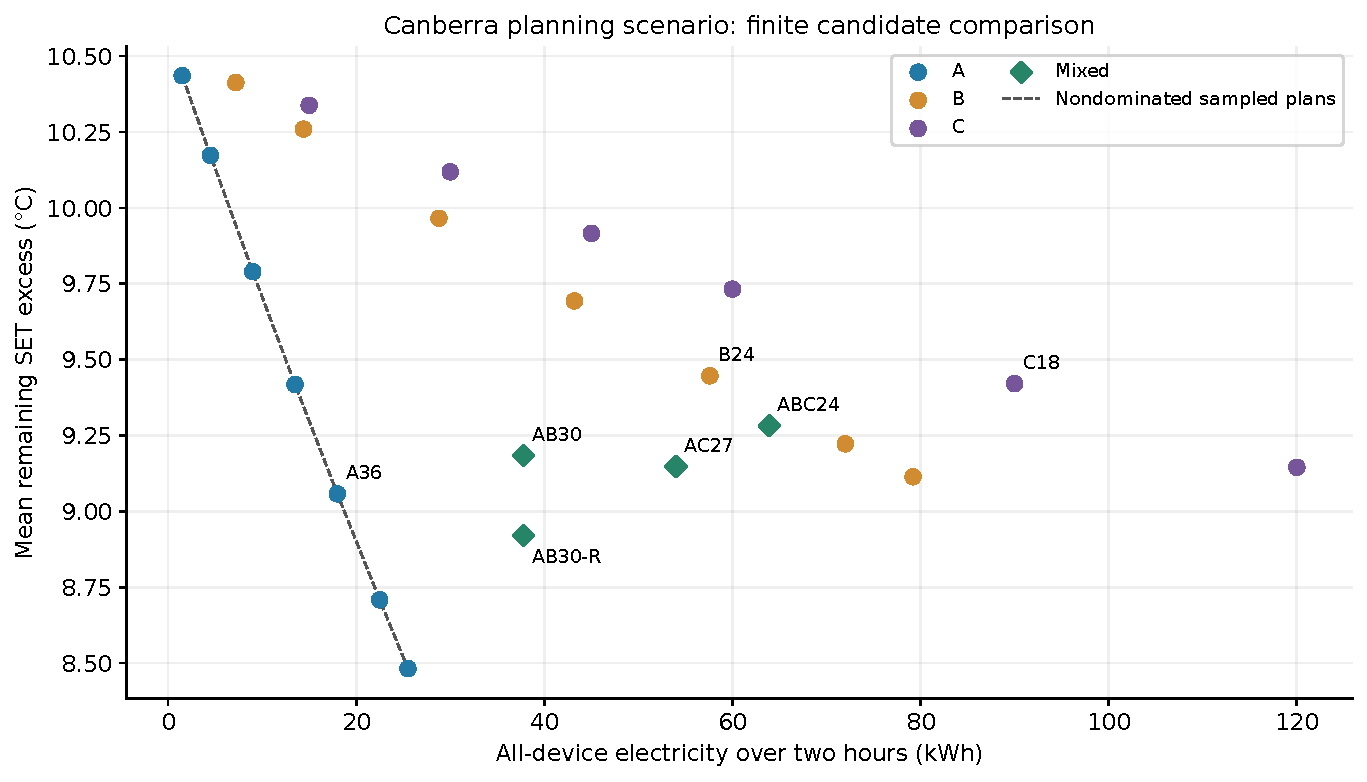
\includegraphics[width=0.90\linewidth]{figures/14_deployment_tradeoff.pdf}
\caption{Energy--discomfort tradeoffs for 24 candidate configurations. The dashed line marks the nondominated candidates; required passenger coverage guides selection.}
\label{fig:deployment-tradeoff}
\end{figure}

\begin{figure}[!ht]
\centering
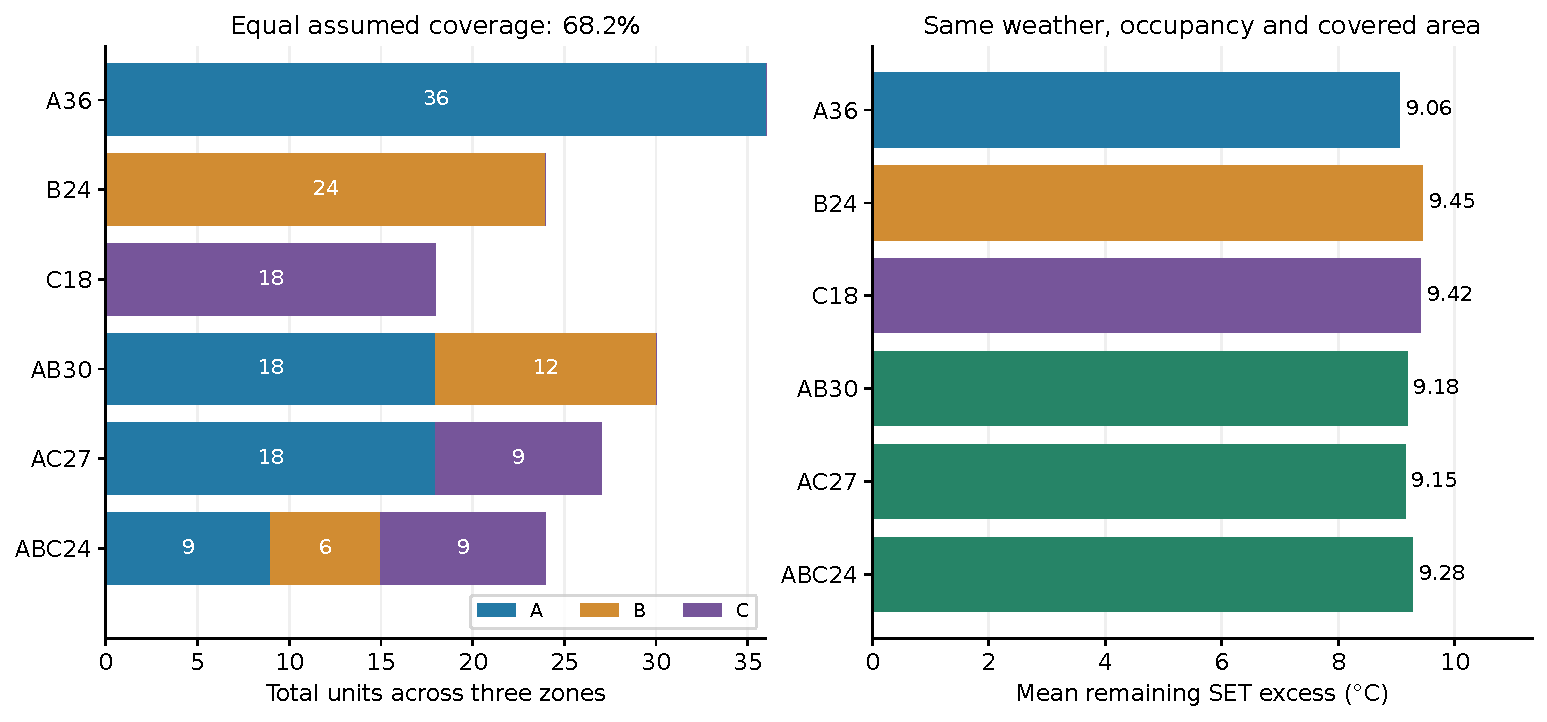
\includegraphics[width=0.90\linewidth]{figures/15_deployment_mix.pdf}
\caption{Equal-footprint deployment comparison: counts and performance at $68.2\%$ direct-service coverage. All devices contribute to the shared heat/moisture balances and total electricity.}
\label{fig:deployment-mix}
\end{figure}

\begin{figure}[!ht]
\centering
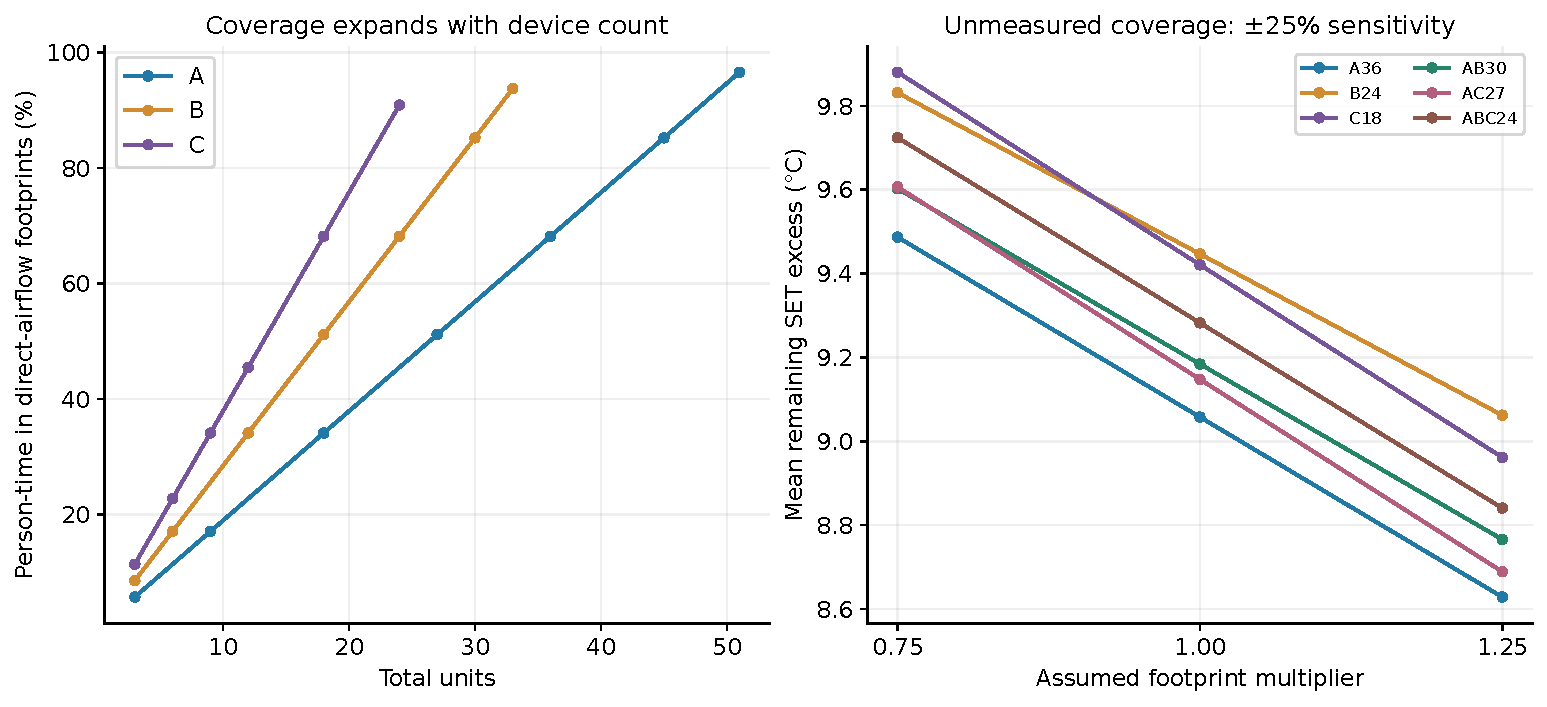
\includegraphics[width=\linewidth]{figures/16_deployment_coverage.pdf}
\caption{Device-count and assumed-footprint sensitivity. Changing footprint affects direct-service fractions; numerical coverage is not a verified equipment rating.}
\label{fig:deployment-coverage}
\end{figure}

\subsection{Usefulness, station-wide transfer, and verification}

By resolving thermal storage, moisture accumulation and changing passenger loads, the revised model links equipment selection to conditions throughout the waiting period.

\noindent\begin{minipage}{\linewidth}
\noindent\textbf{Limits of the planning scale.} The selection results depend on effective platform area, air exchange, device throw and passenger distribution. Field measurements and layout constraints, including electrical capacity, stairs and benches, are needed to specify an installation. Shared zone temperatures and separate service footprints approximate equipment delivery; they do not resolve extra cooling in an evaporative outlet jet. The reported ranking therefore applies to the stated scenario and should be reassessed when these inputs are calibrated.
\end{minipage}

\Needspace{7\baselineskip}
\noindent\textbf{Verification.} RK4 uses a 20 s step aligned with schedule boundaries. Repeating the three mixed benchmarks at 10 s changes efficiency by less than $0.001\%$ and mean remaining SET excess by less than $10^{-5}\,^{\circ}\mathrm C$. Eleven checks cover integer counts, non-overlapping coverage, full electricity, heat/moisture conservation, $U_s+R_s=R_0$, valid psychrometrics and SET, reduction to a pure-device model, zero-occupancy accounting, signed adverse effects, coverage weights and convergence. Maximum candidate energy and vapor residuals are below $4\times10^{-6}$ J and $2\times10^{-13}$ kg. These verify implementation consistency, not field accuracy.

The accompanying \texttt{deployment\_model} folder contains the scenario, solver, CSV trajectories, initial states, sensitivity results and verification records. SET remains a quasi-steady human-response calculation even though the environment is dynamic. The model neglects surface moisture sorption, condensation, detailed stratification and direct solar exposure. It stops on invalid humidity or SET inputs instead of hiding them. Outdoor exchange, effective occupied area and coverage need field calibration before operational recommendations.


\clearpage
\phantomsection
\addcontentsline{toc}{section}{References}
\begin{thebibliography}{99}
\footnotesize
\urlstyle{same}
\setlength{\itemsep}{0pt}
\setlength{\parskip}{0pt}
\bibitem{ashrae}
ASHRAE. \emph{2026 ASHRAE Handbook---Refrigeration},
Chapter 15, \emph{Retail Food Store Refrigeration and Equipment}.
Product Temperatures and Display Refrigerator Cooling Load sections.
\url{https://handbook.ashrae.org/Handbooks/R26/IP/r26_ch15/r26_ch15_ip.aspx}.
Accessed November 7, 2026.

\bibitem{etl}
UK Department for Energy Security and Net Zero.
\emph{Energy Technology List: Retrofit Measures for Open Fronted Refrigerated Display Cabinets}.
Definitions and product-temperature performance requirements.
\url{https://etl.energysecurity.gov.uk/products/refrigeration-equipment/retrofit-measures-open-fronted-refrigerated-display-cabinets}.
Accessed November 7, 2026.

\bibitem{energystar}
ENERGY STAR. \emph{Ceiling Fan Installation and Usage Tips}.
\url{https://www.energystar.gov/products/ceiling_fans/installation-and-usage-tips}.
Accessed November 7, 2026.

\bibitem{evap}
ASHRAE. \emph{2023 ASHRAE Handbook---HVAC Applications},
Chapter 53, \emph{Evaporative Cooling}.
\url{https://handbook.ashrae.org/Handbooks/A23/SI/A23_Ch53/a23_ch53_si.aspx}.
Accessed November 7, 2026.

\bibitem{problem}
COMAP. \emph{2026 HiMCM Problem B: Air Conditioning the Environment: Modeling Energy Waste in Public Cooling}.
User-supplied problem statement, Requirement 2(a), p.~2.

\bibitem{evapequip}
ASHRAE. \emph{2020 ASHRAE Handbook---HVAC Systems and Equipment},
Chapter 41, \emph{Evaporative Air-Cooling Equipment}, Section 1.
\url{https://handbook.ashrae.org/handbooks/S20/SI/s20_ch41/s20_ch41_si.aspx}.
Accessed November 7, 2026.

\bibitem{fanguide}
Center for the Built Environment, University of California, Berkeley.
\emph{Fans for Cooling People Guidebook: Elevated Air Speed and Thermal Comfort}.
\url{https://cbe-berkeley.gitbook.io/fans-guidebook/full-guidebook/elevated-air-speed-and-thermal-comfort}.
Accessed November 7, 2026.

\bibitem{thermalcomfort}
ASHRAE. \emph{2017 ASHRAE Handbook---Fundamentals},
Chapter 9, \emph{Thermal Comfort}, Section 10, Environmental Indices.
\url{https://handbook.ashrae.org/Handbooks/f17/IP/f17_ch09/f17_ch09_ip.aspx}.
Accessed November 7, 2026.

\bibitem{pythermal}
Tartarini, F., and Schiavon, S. (2020).
pythermalcomfort: A Python package for thermal comfort research.
\emph{SoftwareX}, 12, 100578.
\url{https://doi.org/10.1016/j.softx.2020.100578}.
SET API and applicability limits:
\url{https://pythermalcomfort.readthedocs.io/en/stable/documentation/models.html}.
Accessed November 7, 2026.

\bibitem{psychrolib}
Meyer, D., and Thevenard, D. (2019).
PsychroLib: a library of psychrometric functions to calculate thermodynamic properties of air.
\emph{Journal of Open Source Software}, 4(33), 1137.
\url{https://doi.org/10.21105/joss.01137}.
SI psychrometric API:
\url{https://psychrometrics.github.io/psychrolib/api_docs.html}.
Accessed November 7, 2026.

\bibitem{nycshelter}
New York City Department of Transportation.
\emph{Street Design Manual: Bus Stop Shelter}, Description (regular-size shelter).
\url{https://www.nycstreetdesign.info/furniture/bus-stop-shelter}.
Accessed November 7, 2026.

\bibitem{hillphoenix}
Hillphoenix. \emph{CF-R/CF-FS-R/CF-S-R Multi-Deck Merchandiser: Installation \& Operations Manual}, April 2021, Technical Reference, printed p.~4 (PDF p.~8).
\url{https://www.hillphoenix.com/wp-content/uploads/2021/06/CF-S-R-display-case-manual.pdf}.
Product classification: \url{https://www.hillphoenix.com/products/cf}.
Accessed November 7, 2026.

\bibitem{epzone}
EnergyPlus Development Team. \emph{Engineering Reference},
``Basis for the Zone and Air System Integration'' and ``Moisture Predictor-Corrector.''
\href{https://energyplus.readthedocs.io/en/latest/guides/engineering-reference/2.1-basis-for-the-zone-and-air-system-integration.html}{Online source};
\href{https://energyplus.readthedocs.io/en/latest/guides/engineering-reference/2.4-moisture-predictor-corrector.html}{Online source}.
Accessed November 7, 2026.

\bibitem{ventilation}
ASHRAE. \emph{2025 ASHRAE Handbook---Fundamentals}, Chapter 16,
\emph{Ventilation and Infiltration}, Section 10, Natural Ventilation.
\href{https://handbook.ashrae.org/Handbooks/F25/SI/F25_Ch16/F25_Ch16_si.aspx}{Online source}.
Accessed November 7, 2026.

\bibitem{canberra-rsp}
RSP. \emph{Canberra Station}. Project description and site area.
\href{https://rsp.design/project/canberrastation/}{Online source}. Accessed November 7, 2026.

\bibitem{canberra-lta}
Land Transport Authority. \emph{Stations, stations on the tracks, which is the greenest of them all?}
Canberra station: natural ventilation, planting, glazing and louvers.
\href{https://www.lta.gov.sg/content/ltagov/en/who_we_are/statistics_and_publications/Connect/greenmrtstations.html}{Online source}.
Accessed November 7, 2026.

\bibitem{canberra-dimensions}
\emph{The Straits Times}. \emph{Safety first as work starts on new Canberra MRT station on `live' North-South Line}, March 26, 2016.
Source identified in the user-supplied schematic for approximate structural dimensions.
\href{https://www.straitstimes.com/singapore/safety-first-as-work-starts-on-new-canberra-mrt-station-on-live-north-south-line}{Online source}.

\bibitem{singapore-climate}
Meteorological Service Singapore. \emph{Climate of Singapore}. Temperature and humidity climatology.
\href{https://www.weather.gov.sg/climate-climate-of-singapore}{Online source}. Accessed November 7, 2026.

\bibitem{gemini}
Google Gemini. \emph{AI-generated analysis of the 2026 HiMCM Problem B},
user-supplied PDF conversation excerpt, November 2026.
Consulted for process-oriented exposition; the proposed efficiency formula was
reviewed but not adopted. Exact model identifier was not available in the supplied excerpt.

\bibitem{codex}
OpenAI. \emph{Codex}, AI-assisted formulation, reference checking,
English drafting, and LaTeX preparation, November 2026.
Exact deployed model identifier to be recorded from the session interface.
See the preliminary AI-use record following this draft.

\bibitem{aipolicy}
COMAP. \emph{Use of AI Tools in COMAP Contests}, v102025.
\url{https://www.contest.comap.com/undergraduate/contests/mcm/flyer/Contest_AI_Policy.pdf}.
Accessed November 7, 2026.
\end{thebibliography}

% Add Requirements 3--5, the memorandum, and the blog before References.
% Replace the working summary after completing the full analysis.
\clearpage
\phantomsection
\addcontentsline{toc}{section}{Report on Use of AI Tools}
\section*{Report on Use of AI Tools}
\noindent\textbf{Preliminary record for this partial draft.}

OpenAI Codex assisted with translation, modeling, coding and drafting Requirements
1 and 2 in November 2026. Record the exact deployed model identifier from the session interface.

For Requirement 1, the user requested indicator justification and transfer from
refrigerated storage to public cooling. This is a request summary, not a transcript.

Codex simplified the evaluation framework, checked sources, drafted the text,
and prepared the LaTeX. AI review checked technical consistency. At the user's request,
the 2025 Problem B solutions of Teams 16442, 16738, and 16739 were reviewed as
structural references. Their numerical estimates, weighting procedures, and
wording were not used in the present model. No field measurements or empirical
performance results were produced.

A user-supplied Google Gemini conversation excerpt was subsequently reviewed.
Its process-oriented explanation informed the organization of the new diagram;
Codex redrew and revised the dependencies and service definitions. The Gemini
model identifier and complete conversation were not available in that excerpt.
The relevant Gemini prompts and outputs must also be included in the final record.

For Requirement 2(a), the user requested the bus-stop extension, citations and
charts. Codex formulated the three-zone scenario, wrote Python code using
PsychroLib and pythermalcomfort, generated six figures and CSV results, and
drafted the interpretation. AI review checked physical assumptions, sources,
and equation/code consistency. Delivery profiles remain assumptions; numerical
checks do not establish field accuracy. Software versions accompany the results.

Codex incorporated the user's bus-shelter schematic, checked NYC dimensions,
adopted them for equal zones, updated occupancy accounting and geometry checks,
and generated a PDF zoning diagram. Original image pixels were preserved; the
page viewport was adjusted for caption numbering and attribution.

A second user-supplied schematic of an open refrigerated display case was
incorporated into Requirement 1 as a separate PDF. Codex checked the model
classification and dimensions against the manufacturer's material, added source
attribution and a structural explanation, and preserved the original image.
The figure illustrates geometry; no freezer performance data were inferred.

For Requirement 2(b), Codex developed coupled zone enthalpy, moisture and
surface-energy balances, implemented a dynamic station scenario, and generated
three separate PDF figures. AI review checked conservation, vapor-source
accounting, source support, and numerical consistency. Geometry, equipment
flows and train/passenger schedules remain explicit scenario assumptions.
The work did not include field measurements or empirical model validation.

For the Canberra revision, Codex incorporated the user's station schematic and checked architectural and climate sources. Codex developed variable device counts, allocation and coverage, simulated candidate configurations, and revised the discussion around service requirements and equipment selection. Area, device footprints and operating conditions remain assumptions; no installed equipment inventory or field performance is claimed.

Before submission, add exact relevant prompts and complete outputs for all
retained contributions and AI tools, following the contest guidance \cite{aipolicy}.
Retain this source and chat as records. Independent student verification has
not been asserted in this preliminary record.

\end{document}

